
The limits for the cut based VBF channel are shown in 
Table~\ref{tab:uls_2j_cut} and Figure~\ref{fig:uls_2j_cut}.
The limits for the cut based analysis in all final states are shown in
Table~\ref{tab:ulscut} and Figure~\ref{fig:uls_cut}.
The BDT and 2D analyses in the 0 and 1-jet different flavor final states
are combined with the cut based VBF and same flavor analyses in
Tables~\ref{tab:uls_bdt01_cut2_cutsf} and~\ref{tab:uls_2d01_cut2_cutsf}
and Figures~\ref{fig:uls_bdt01_cut2_cutsf} and~\ref{fig:uls_2d01_cut2_cutsf} 
respectively.

%%%%%%%%%%%%%%%%%
% plot
\begin{figure}[!hbtp]
\centering
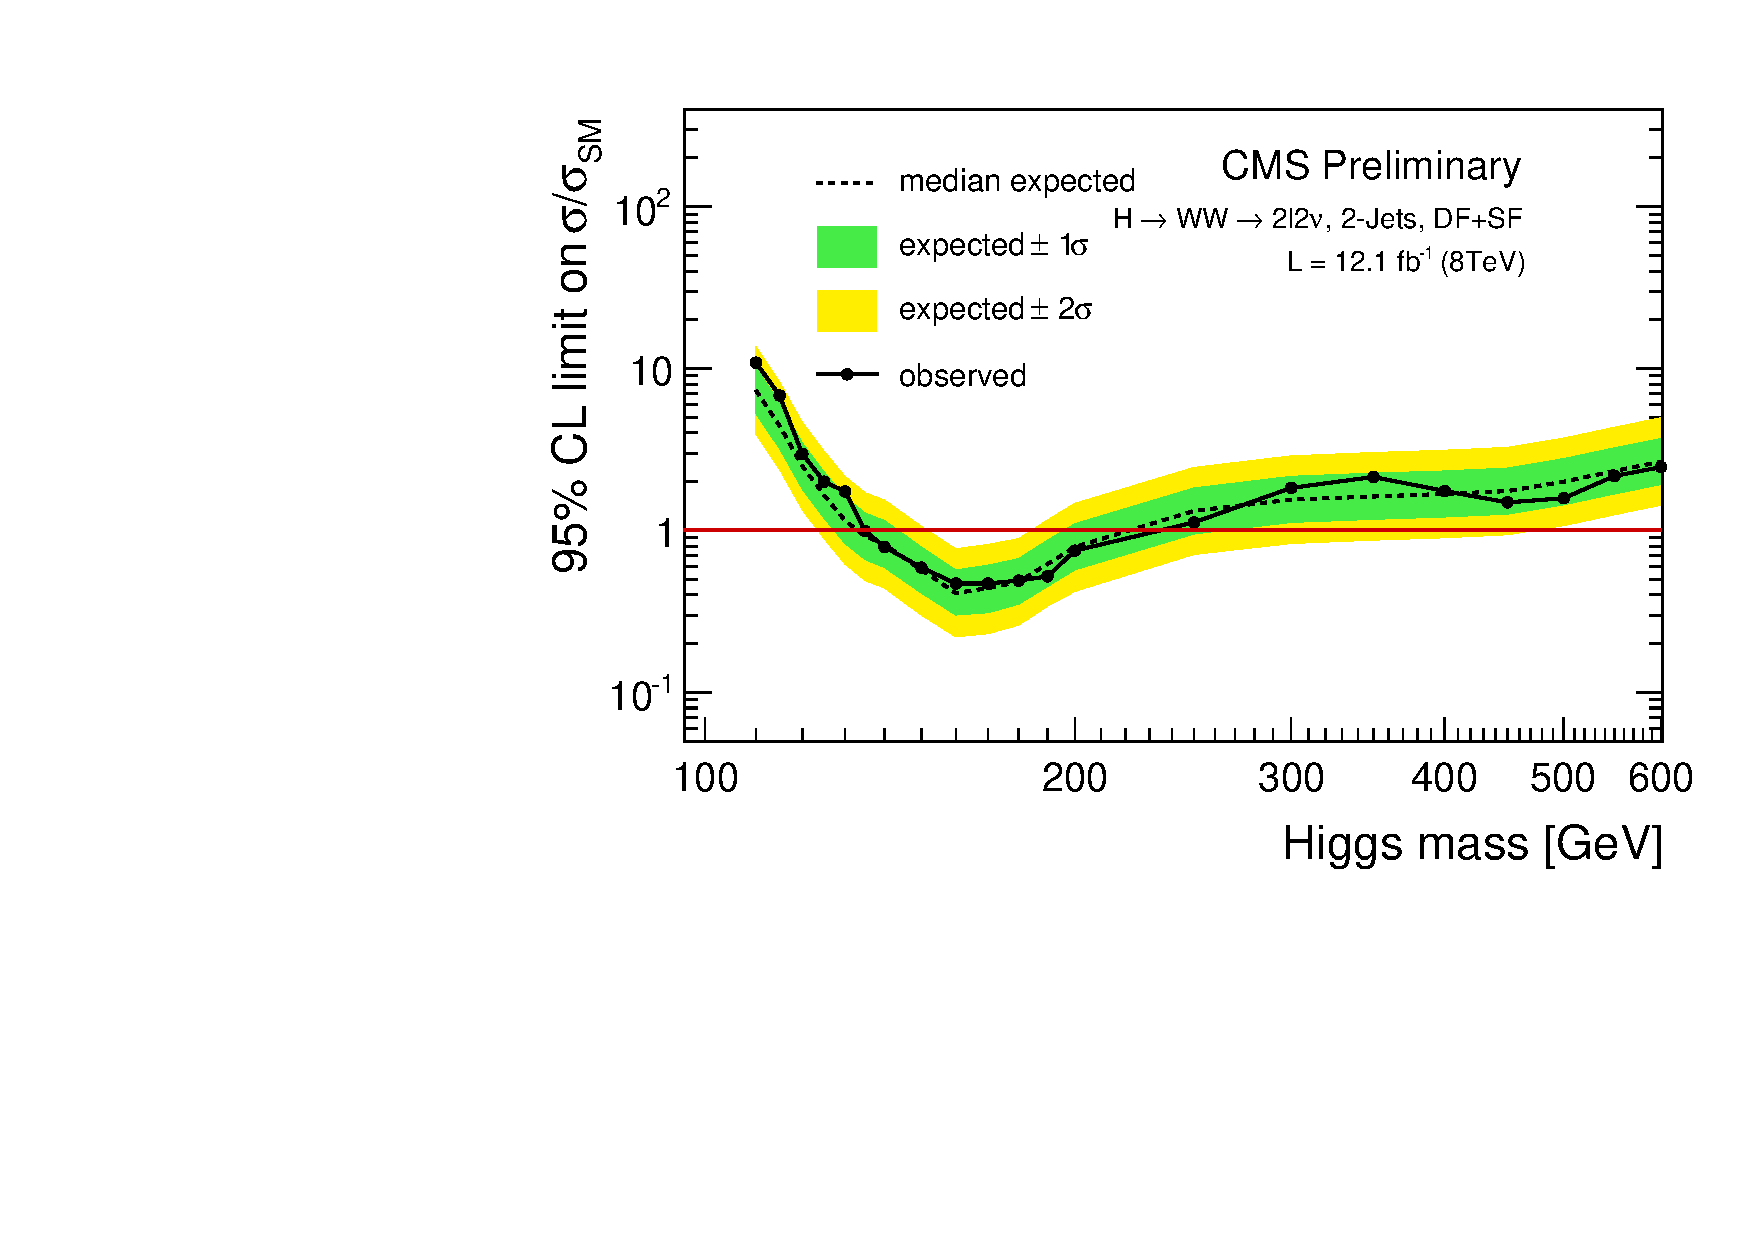
\includegraphics[width=.75\textwidth]{figures/table_limits_2j_cut_log.pdf}
\caption{Expected upper limits for SM Higgs in $\intlumiEightTeV$ at 8 TeV in the VBF channel.
The cut-based result is used. }
\label{fig:uls_2j_cut}
\end{figure}
% table
\begin{table}[!htbp]
\begin{center}
\begin{tabular}{c c c c c}
\hline
\vspace{-3mm} && \\
Higgs Mass & Observed  & Median expected & Expected range for 68\% & Expected range for 95\%   \\
\hline
110 & -1.00 & 7.40 & [5.33, 10.29] & [3.97, 13.80] \\
115 & -1.00 & 4.72 & [3.40, 6.57] & [2.53, 8.81] \\
120 & -1.00 & 2.52 & [1.81, 3.50] & [1.35, 4.70] \\
125 & -1.00 & 1.67 & [1.20, 2.33] & [0.90, 3.12] \\
130 & -1.00 & 1.15 & [0.83, 1.60] & [0.62, 2.15] \\
135 & -1.00 & 0.93 & [0.67, 1.30] & [0.50, 1.74] \\
140 & -1.00 & 0.83 & [0.60, 1.15] & [0.44, 1.54] \\
150 & -1.00 & 0.57 & [0.41, 0.79] & [0.30, 1.06] \\
160 & -1.00 & 0.41 & [0.30, 0.57] & [0.22, 0.77] \\
170 & -1.00 & 0.44 & [0.31, 0.61] & [0.23, 0.82] \\
180 & -1.00 & 0.48 & [0.35, 0.67] & [0.26, 0.90] \\
190 & -1.00 & 0.63 & [0.45, 0.88] & [0.34, 1.18] \\
200 & -1.00 & 0.81 & [0.58, 1.12] & [0.43, 1.50] \\
250 & -1.00 & 1.35 & [0.97, 1.88] & [0.72, 2.52] \\
300 & -1.00 & 1.57 & [1.13, 2.19] & [0.85, 2.94] \\
350 & -1.00 & 1.62 & [1.17, 2.26] & [0.87, 3.03] \\
400 & -1.00 & 1.68 & [1.21, 2.33] & [0.90, 3.13] \\
450 & -1.00 & 1.75 & [1.26, 2.43] & [0.94, 3.26] \\
500 & -1.00 & 2.00 & [1.44, 2.78] & [1.07, 3.72] \\
550 & -1.00 & 2.33 & [1.68, 3.24] & [1.25, 4.34] \\
600 & -1.00 & 2.66 & [1.92, 3.70] & [1.43, 4.97] \\
\vspace{-3mm} && \\
\hline
\end{tabular}
\caption{Expected upper limits for SM Higgs in $\intlumiEightTeV$ at 8 TeV in the VBF channel.
The cut-based result is used. }
\label{tab:uls_2j_cut}
\end{center}
\end{table}
%%%%%%%%%%

%%%%%%%%%%%%%%%%%
% plot
\begin{figure}[!hbtp]
\centering
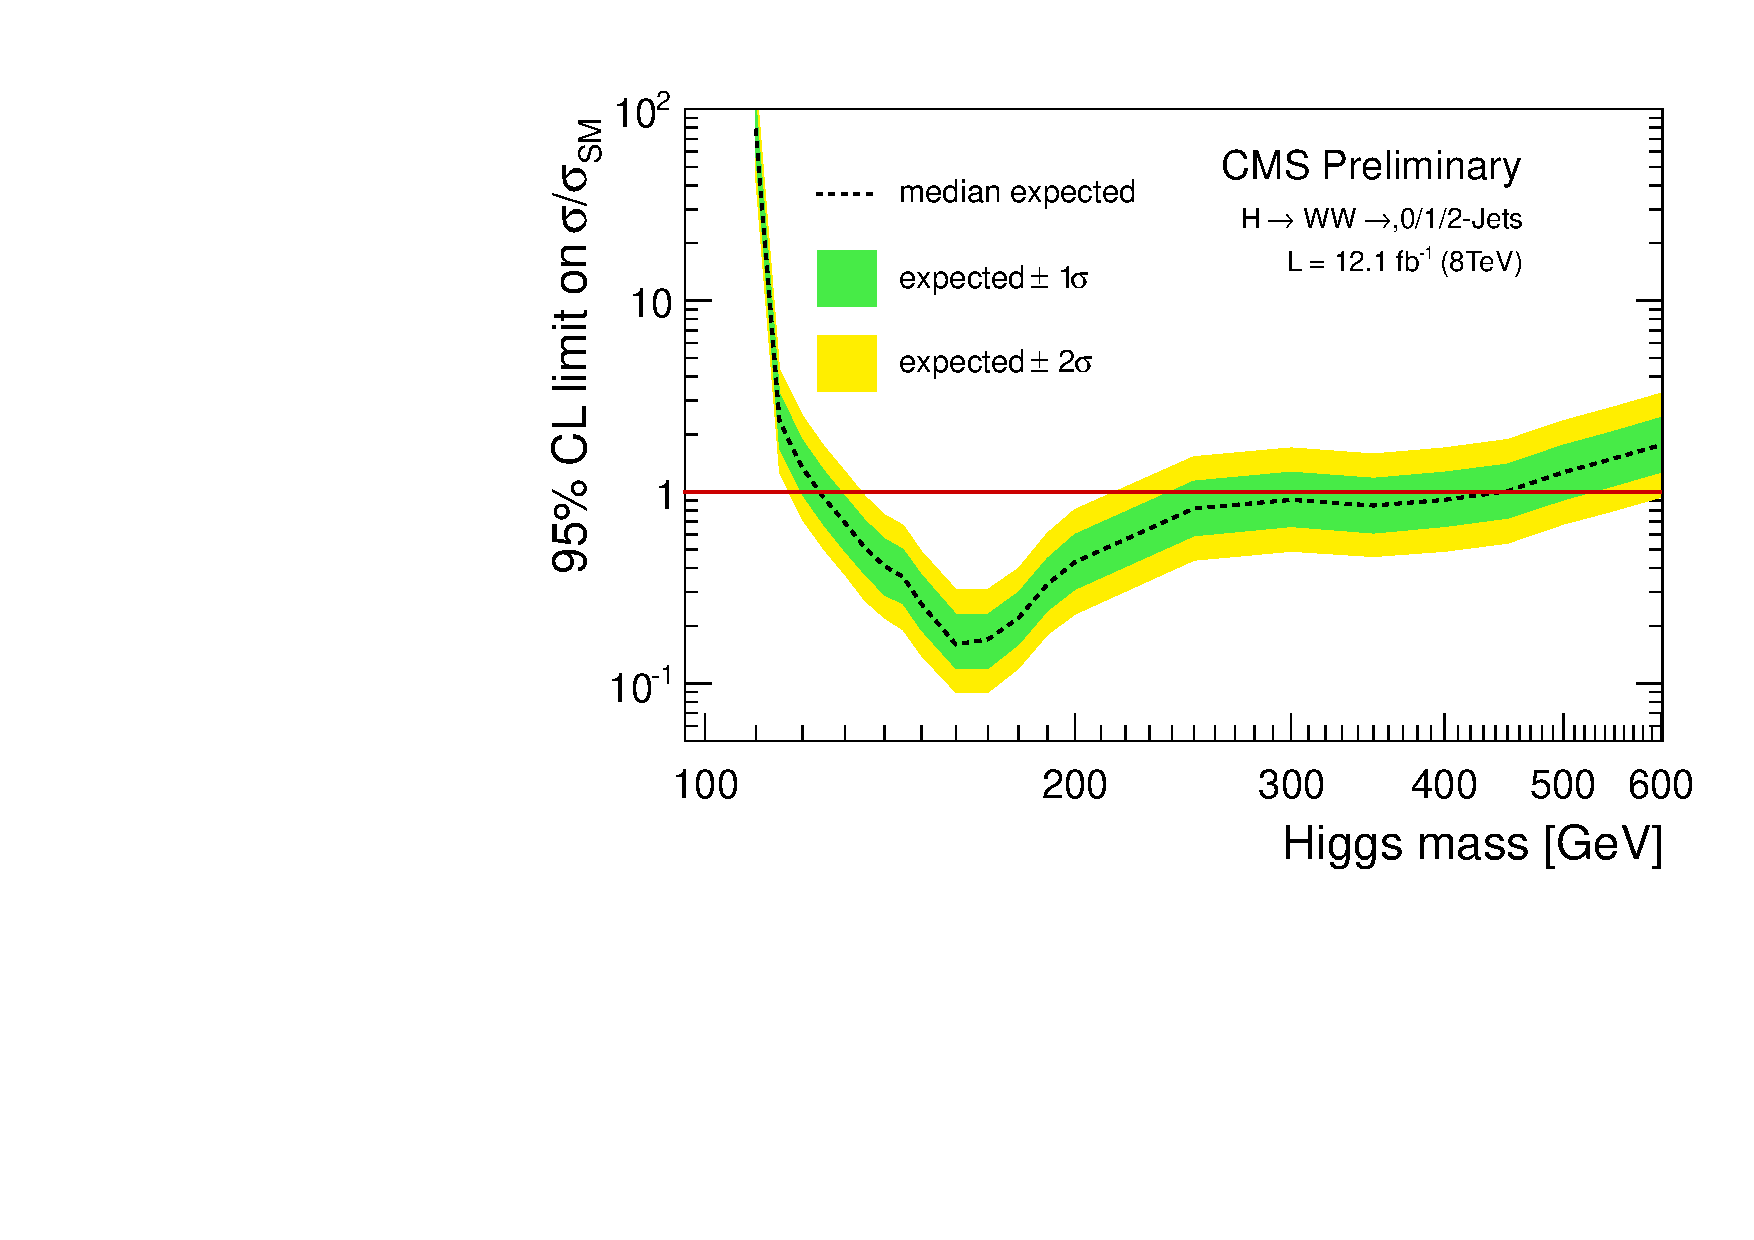
\includegraphics[width=.75\textwidth]{figures/table_limits_nj_cut_log.pdf}
\caption{Expected upper limits for SM Higgs in $\intlumiEightTeV$ at 8 TeV in all final states combined.
Cut-based result is used. }
\label{fig:uls_cut}
\end{figure}
% table
\begin{table}[!htbp]
\begin{center}
\begin{tabular}{c c c c c}
\hline
\vspace{-3mm} && \\
Higgs Mass & Observed  & Median expected & Expected range for 68\% & Expected range for 95\%   \\
\hline
110 & -1.00 & 4.26 & [3.07, 5.93] & [2.29, 7.96] \\
115 & -1.00 & 2.17 & [1.56, 3.01] & [1.16, 4.04] \\
120 & -1.00 & 1.26 & [0.91, 1.75] & [0.68, 2.35] \\
125 & -1.00 & 0.87 & [0.63, 1.21] & [0.47, 1.62] \\
130 & -1.00 & 0.65 & [0.47, 0.90] & [0.35, 1.21] \\
135 & -1.00 & 0.48 & [0.35, 0.67] & [0.26, 0.90] \\
140 & -1.00 & 0.39 & [0.28, 0.55] & [0.21, 0.73] \\
150 & -1.00 & 0.26 & [0.19, 0.36] & [0.14, 0.49] \\
160 & -1.00 & 0.16 & [0.12, 0.23] & [0.09, 0.31] \\
170 & -1.00 & 0.17 & [0.12, 0.23] & [0.09, 0.31] \\
180 & -1.00 & 0.22 & [0.16, 0.30] & [0.12, 0.40] \\
190 & -1.00 & 0.33 & [0.24, 0.45] & [0.18, 0.61] \\
200 & -1.00 & 0.44 & [0.31, 0.61] & [0.23, 0.81] \\
250 & -1.00 & 0.82 & [0.59, 1.14] & [0.44, 1.53] \\
300 & -1.00 & 0.92 & [0.66, 1.28] & [0.49, 1.71] \\
350 & -1.00 & 0.84 & [0.61, 1.18] & [0.45, 1.58] \\
400 & -1.00 & 0.90 & [0.65, 1.25] & [0.48, 1.68] \\
450 & -1.00 & 0.99 & [0.72, 1.38] & [0.53, 1.85] \\
500 & -1.00 & 1.24 & [0.89, 1.72] & [0.66, 2.31] \\
550 & -1.00 & 1.47 & [1.06, 2.04] & [0.79, 2.74] \\
600 & -1.00 & 1.69 & [1.22, 2.36] & [0.91, 3.16] \\
\vspace{-3mm} && \\
\hline
\end{tabular}
\caption{Expected upper limits for SM Higgs in $\intlumiEightTeV$ at 8 TeV in all final states combined.
Cut-based result is used. }
\label{tab:ulscut}
\end{center}
\end{table}
%%%%%%%%%%

%%%%%%%%%%%%%%%%%
% plot
\begin{figure}[!hbtp]
\centering
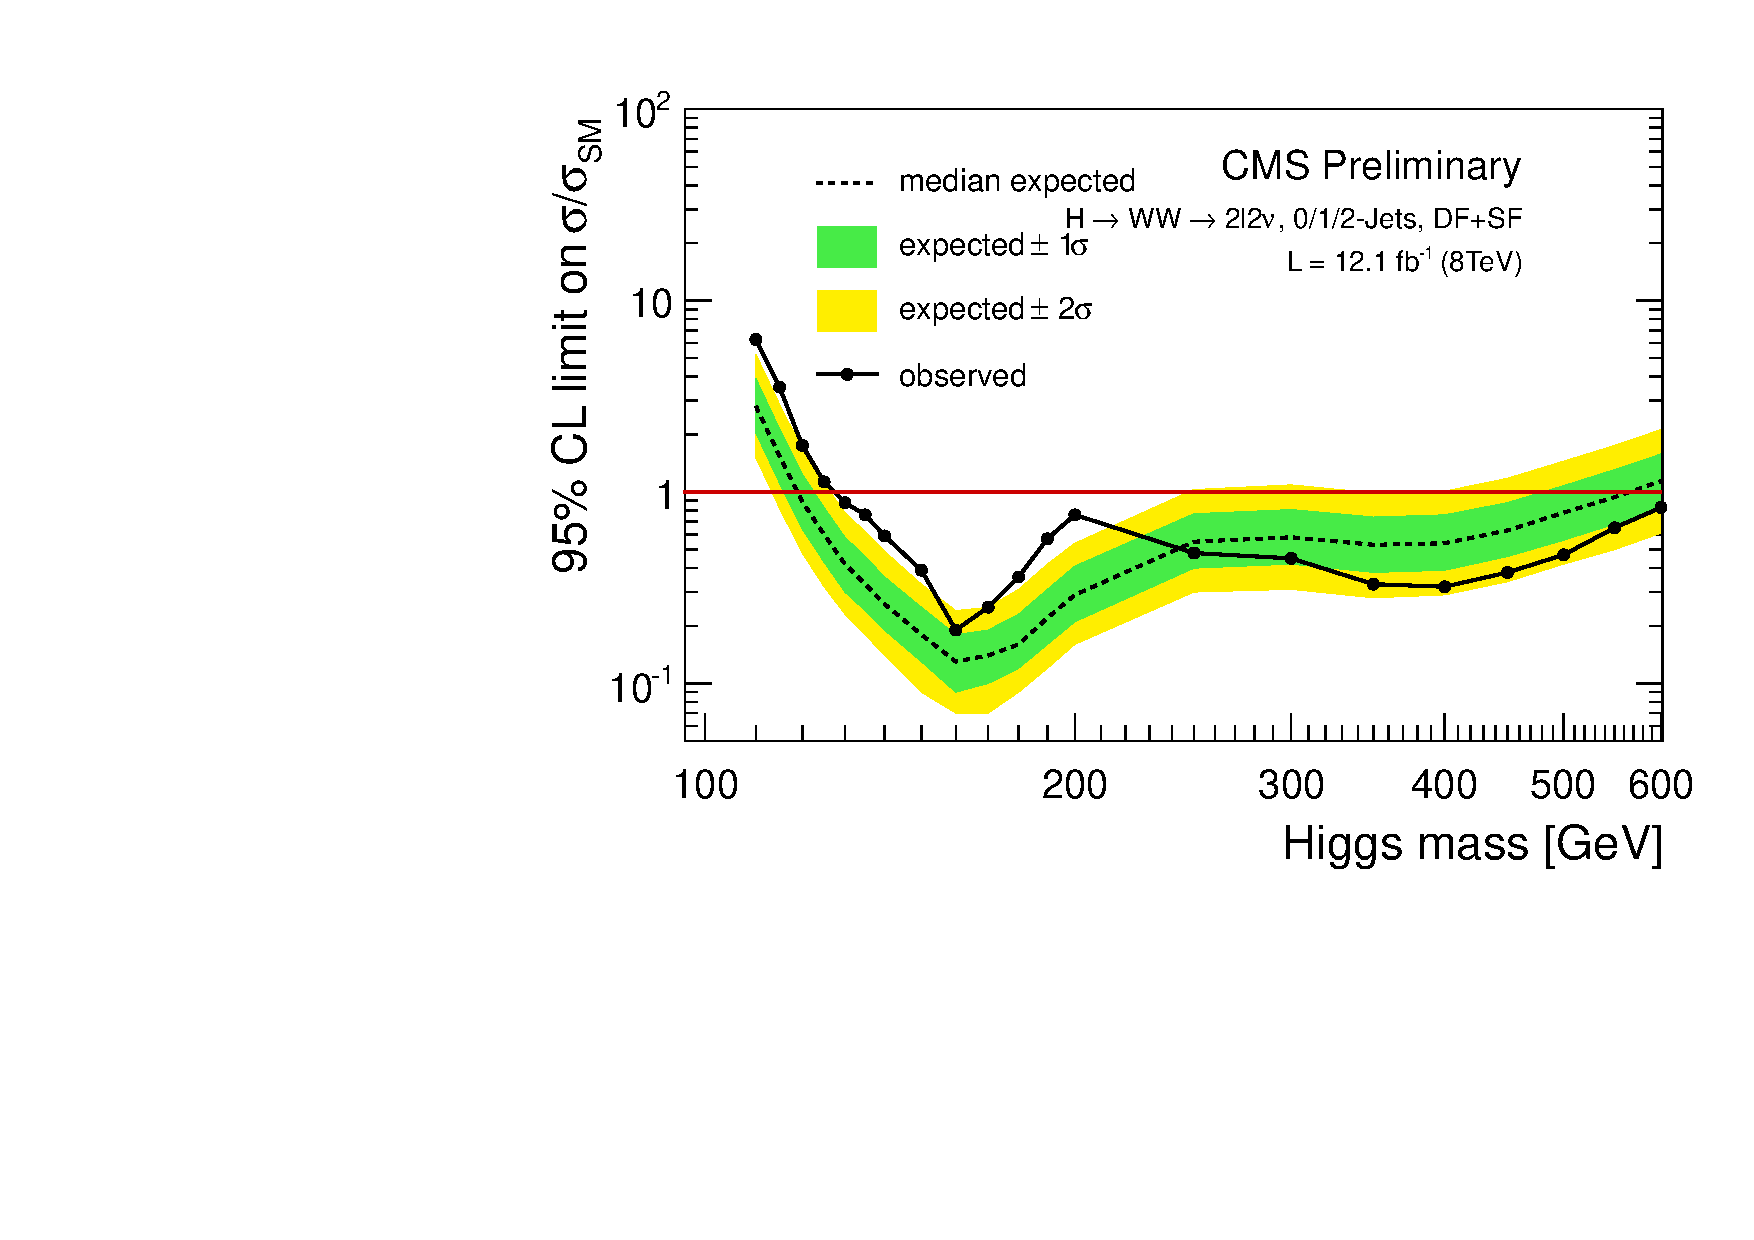
\includegraphics[width=.75\textwidth]{figures/table_limits_nj_shapebdt_of_cut_sf_log.pdf}
\caption{Expected upper limits for SM Higgs in $\intlumiEightTeV$ at 8 TeV.
BDT result is used for OF 0/1jet bin and cut-based result is used for VBF channel
and in the SF final states. }
\label{fig:uls_bdt01_cut2_cutsf}
\end{figure}
% table
\begin{table}[!htbp]
\begin{center}
\begin{tabular}{c c c c c}
\hline
\vspace{-3mm} && \\
Higgs Mass & Observed  & Median expected & Expected range for 68\% & Expected range for 95\%   \\
\hline
110 & -1.00 & 3.09 & [2.22, 4.30] & [1.66, 5.76] \\
115 & -1.00 & 1.58 & [1.14, 2.20] & [0.85, 2.96] \\
120 & -1.00 & 0.92 & [0.66, 1.28] & [0.49, 1.72] \\
125 & -1.00 & 0.62 & [0.45, 0.87] & [0.33, 1.16] \\
130 & -1.00 & 0.44 & [0.31, 0.61] & [0.23, 0.81] \\
135 & -1.00 & 0.36 & [0.26, 0.49] & [0.19, 0.66] \\
140 & -1.00 & 0.27 & [0.19, 0.38] & [0.14, 0.50] \\
150 & -1.00 & 0.18 & [0.13, 0.25] & [0.10, 0.33] \\
160 & -1.00 & 0.13 & [0.09, 0.18] & [0.07, 0.24] \\
170 & -1.00 & 0.14 & [0.10, 0.19] & [0.07, 0.25] \\
180 & -1.00 & 0.16 & [0.12, 0.23] & [0.09, 0.31] \\
190 & -1.00 & 0.22 & [0.16, 0.31] & [0.12, 0.42] \\
200 & -1.00 & 0.29 & [0.21, 0.41] & [0.16, 0.55] \\
250 & -1.00 & 0.56 & [0.40, 0.77] & [0.30, 1.04] \\
300 & -1.00 & 0.58 & [0.42, 0.81] & [0.31, 1.09] \\
350 & -1.00 & 0.53 & [0.38, 0.74] & [0.28, 0.99] \\
400 & -1.00 & 0.54 & [0.39, 0.76] & [0.29, 1.02] \\
450 & -1.00 & 0.63 & [0.46, 0.88] & [0.34, 1.18] \\
500 & -1.00 & 0.78 & [0.56, 1.09] & [0.42, 1.45] \\
550 & -1.00 & 0.94 & [0.68, 1.31] & [0.50, 1.76] \\
600 & -1.00 & 1.14 & [0.82, 1.58] & [0.61, 2.12] \\
\vspace{-3mm} && \\
\hline
\end{tabular}
\caption{Expected upper limits for SM Higgs in $\intlumiEightTeV$ at 8 TeV.
BDT result is used for OF 0/1jet bin and cut-based result is used for VBF channel
and in the SF final states. }
\label{tab:uls_bdt01_cut2_cutsf}
\end{center}
\end{table}
%%%%%%%%%%

%%%%%%%%%%%%%%%%%
% plot
\begin{figure}[!hbtp]
\centering
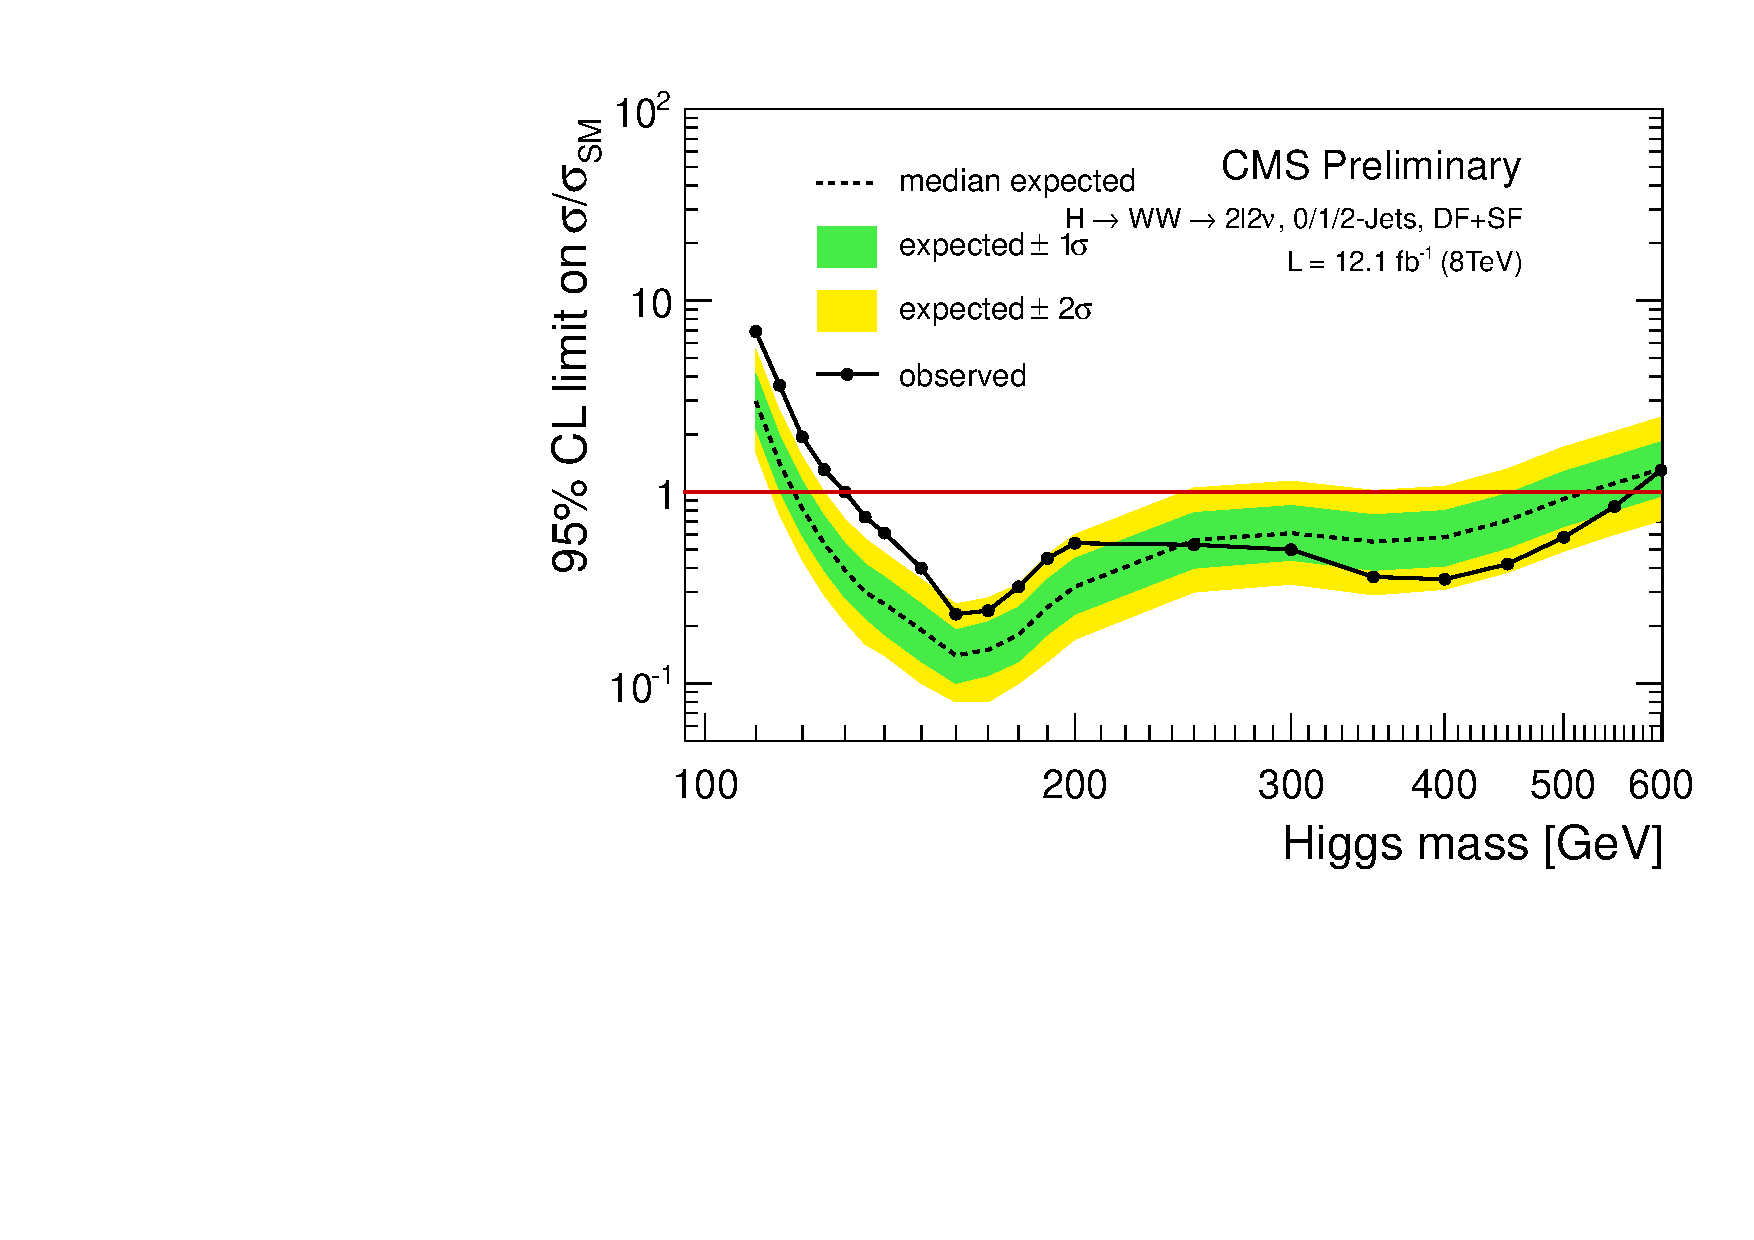
\includegraphics[width=.75\textwidth]{figures/table_limits_nj_shape2d_of_cut_sf_log.pdf}
\caption{Expected upper limits for SM Higgs in $\intlumiEightTeV$ at 8 TeV.
2D result is used for OF 0/1jet bin and cut-based result is used for VBF channel
and in the SF final states. }
\label{fig:uls_2d01_cut2_cutsf}
\end{figure}
% table
\begin{table}[!htbp]
\begin{center}
\begin{tabular}{c c c c c}
\hline
\vspace{-3mm} && \\
Higgs Mass & Observed  & Median expected & Expected range for 68\% & Expected range for 95\%   \\
\hline
110 & -1.00 & 3.03 & [2.18, 4.22] & [1.63, 5.66] \\
115 & -1.00 & 1.46 & [1.05, 2.03] & [0.78, 2.72] \\
120 & -1.00 & 0.84 & [0.60, 1.17] & [0.45, 1.56] \\
125 & -1.00 & 0.55 & [0.40, 0.77] & [0.30, 1.03] \\
130 & -1.00 & 0.40 & [0.29, 0.55] & [0.21, 0.74] \\
135 & -1.00 & 0.32 & [0.23, 0.44] & [0.17, 0.59] \\
140 & -1.00 & 0.26 & [0.19, 0.36] & [0.14, 0.49] \\
150 & -1.00 & 0.19 & [0.14, 0.26] & [0.10, 0.35] \\
160 & -1.00 & 0.14 & [0.10, 0.20] & [0.08, 0.26] \\
170 & -1.00 & 0.15 & [0.11, 0.21] & [0.08, 0.28] \\
180 & -1.00 & 0.18 & [0.13, 0.25] & [0.10, 0.33] \\
190 & -1.00 & 0.25 & [0.18, 0.35] & [0.13, 0.47] \\
200 & -1.00 & 0.32 & [0.23, 0.45] & [0.17, 0.60] \\
250 & -1.00 & 0.56 & [0.41, 0.78] & [0.30, 1.05] \\
300 & -1.00 & 0.61 & [0.44, 0.85] & [0.33, 1.14] \\
350 & -1.00 & 0.54 & [0.39, 0.76] & [0.29, 1.02] \\
400 & -1.00 & 0.58 & [0.42, 0.80] & [0.31, 1.07] \\
450 & -1.00 & 0.71 & [0.51, 0.98] & [0.38, 1.32] \\
500 & -1.00 & 0.92 & [0.66, 1.28] & [0.49, 1.72] \\
550 & -1.00 & 1.11 & [0.80, 1.55] & [0.60, 2.07] \\
600 & -1.00 & 1.32 & [0.95, 1.83] & [0.71, 2.46] \\
\vspace{-3mm} && \\
\hline
\end{tabular}
\caption{Expected upper limits for SM Higgs in $\intlumiEightTeV$ at 8 TeV.
2D result is used for OF 0/1jet bin and cut-based result is used for VBF channel
and in the SF final states. }
\label{tab:uls_2d01_cut2_cutsf}
\end{center}
\end{table}
%%%%%%%%%%



